% Created 2021-04-10 Sat 10:56
% Intended LaTeX compiler: pdflatex
\documentclass[11pt]{article}
\usepackage[utf8]{inputenc}
\usepackage[T1]{fontenc}
\usepackage{graphicx}
\usepackage{grffile}
\usepackage{longtable}
\usepackage{wrapfig}
\usepackage{rotating}
\usepackage[normalem]{ulem}
\usepackage{amsmath}
\usepackage{textcomp}
\usepackage{amssymb}
\usepackage{capt-of}
\usepackage{hyperref}
\author{Prashant Tak}
\date{\today}
\title{Blog Source File}
\hypersetup{
 pdfauthor={Prashant Tak},
 pdftitle={Blog Source File},
 pdfkeywords={},
 pdfsubject={},
 pdfcreator={Emacs 28.0.50 (Org mode 9.5)}, 
 pdflang={English}}
\begin{document}

\maketitle
\tableofcontents \clearpage

\section{TODO}
\label{sec:org0cc4585}
\begin{enumerate}
\item Fix Time
\item Add Sections
\item Link to RSS feed
\item Add dark mode toggle
\item \sout{Look into whether latex can be used and generated properly for displaying notes} Improve mathjax performance
\item Create Tufte Theme for hugo that ACTUALLY works based on tufte css and the current tale theme
\item \sout{Replace with material scroll bar}
\item Open external links in new tab by default, unless it's meta-links.
\item Improve Image filter sigh
\end{enumerate}
\section{Doubts}
\label{sec:org56d9ae2}
\begin{enumerate}
\item What is r?
\item dev-corpus refers to?
\item F1 score? Measure of accuracy
\item xpos?
\end{enumerate}

\section{About}
\label{sec:org872d5c7}
Hi! I'm Prashant.

\section{Blog}
\label{sec:org9940d7a}
\subsection{Morphosyntactic Tagging with a Meta-BiLSTM Model - An Overview}
\label{sec:org44dbf12}
(Subtitle: \emph{I had shingles, which is a painful disease.})
\begin{center}
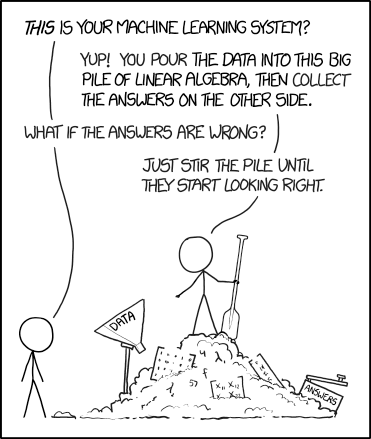
\includegraphics[width=.9\linewidth]{assets/machine_learning.png}
\end{center}

This post contains a complete overview of the titled paper and provides a basic outline of related concepts. This paper aims to investigate to what extent having initial sub-word and word context insensitive representations affect performance.

\subsubsection{Abstract}
\label{sec:orgd64333f}
\begin{enumerate}
\item RNN leads to advances in speech tagging accuracy \href{https://www.aclweb.org/anthology/K18-2001.pdf}{Zeman et al}
\item Common thing among models, \emph{rich initial word encodings}.
\item Encodings are composed of recurrent character-based representation with learned and pre-trained word embeddings\footnote{\href{https://medium.com/@b.terryjack/nlp-everything-about-word-embeddings-9ea21f51ccfe}{Everything about Embeddings} Embedding converts symbolic representations into meaningful numbers}.
\item Problem with the encodings, context restriced to a single word hence only via subsequent recurrent layers the word information is processed.
\item The paper deals with models that use RNN with sentence-level context.
\item This provides results via synchronized training with a meta-model that learns to combine their states.
\item Results are provided on part-of-speech and morphological tagging\footnote{Morphological tagging is the task of assigning labels to a sequence of tokens that describe them morphologically. As compared to Part-of-speech tagging, morphological tagging also considers morphological features, such as case, gender or the tense of verbs.} with great performance on a number of languages.
\end{enumerate}
\subsubsection{Terms}
\label{sec:org3afccf1}
\begin{enumerate}
\item Morphosyntactic = Morphology + Syntax and Morphology is study of words, how they are formed, and their relationship to other words in the same language.
\item \href{https://medium.datadriveninvestor.com/how-do-lstm-networks-solve-the-problem-of-vanishing-gradients-a6784971a577}{RNN}: \href{https://arxiv.org/pdf/1211.5063.pdf}{On difficulty of training RNNs}
\item \href{http://colah.github.io/posts/2015-08-Understanding-LSTMs/}{LSTM}: Long Short-Term Memory is a type of RNN that addresses the vanishing gradient problem through additional cells, input and output gates.
\item BiLSTM: It is a sequence processing model that consists of two LSTMs. They effectively increase the amount of information available to the network, improving the context available to the algorithm (e.g. knowing what words immediately follow and precede a word in a sentence).
\end{enumerate}
\subsubsection{\href{https://www.kdnuggets.com/2018/06/getting-started-natural-language-processing.html}{Basics of NLP} / Pre-requisites}
\label{sec:org0e6bb42}
\begin{enumerate}
\item Key Terms
\label{sec:org6318b85}
\begin{enumerate}
\item \textbf{NLP}: Natural Language Processing concerns itself with interaction of technology with human languages.
\item \textbf{Tokenization}: An early step in the NLP process which splits longer strings of text into smaller pieces, or \emph{tokens}.
\item \textbf{Normalization}: A series of tasks meant to put all text on a level playing field i.e. converting it to lowercase, removing punctuation, expanding contractions, converting numbers to their word equivalents, stripping white space, removing stop words and so on.
\begin{itemize}
\item \textbf{Stemming}: Process of eliminating affixes (suffixes, prefixes, infixes, circumfixes) from a word to obtain its stem. For example, \emph{running} becomes \emph{run}.
\item \textbf{Lemmatization}: It's related to stemming but is able to capture canonical forms based on the word's lemma (root form). For example, \emph{better} would turn into \emph{good}.
\end{itemize}
\item \textbf{Corpus}: The latin word for \emph{body} refers to a collection of texts which may be formed of a single language of texts, or multiple. They are generally used for statistical linguistic analysis and hypothesis testing.
\item \textbf{Stop words}: Filter words which contribute little to the overall meaning of text since they are the very common words of the language. For example: \emph{the}, \emph{a} etc.
\item \textbf{Parts-of-speech (POS) Tagging}: It consists of assigning a category tag to the tokenized parts of a sentence such as nouns, verbs, adjectives etc. The category of words is distinguished since they share similar grammatical properties.
\item \textbf{Statistical Language Modeling}: It's the process of building a model which takes \emph{words} as input and assign probabilities to the various sequences that can be formed using them.
\item \textbf{Bag of words}: It's a representation model used to simplify the contents of a selection of text by just reducing the words to their frequency.
\item \textbf{n-gram}: It focuses on preserving contagious sequences of N items from the text selection.
\end{enumerate}
\item A framework for NLP
\label{sec:org70ac094}
\begin{enumerate}
\item \textbf{Data Collection or Assembly}: Building the corpus
\item \textbf{Data Preprocessing}: Perform operations on the collected corpus which consists of tokenization, normalization, substitution (noise removal).
\item \textbf{Data Exploration \& Visualization}: Includes visualizing word counts and distributions, generating wordclouds, performing distance measures.
\item \textbf{Model Building}: Choosing the language models (FSM, MM), classifiers and sequence models (RNNs, LSTMs).
\item \textbf{Model Evaluation}
\end{enumerate}
\item Data Representation
\label{sec:org3f034a5}
\begin{enumerate}
\item We need to encode text in a way that can be controlled by us using a statistical classifier.
\item We go from a set of categorical features in text: words, letters, POS tags, word arrangement, order etc to a series of \emph{vectors}.
\item \textbf{One-hot Encoding} (Sparse Vectors) :
\begin{itemize}
\item Each word, or token corresponds to a vector element.
\item Result of one-hot encoding is a sparse matrix, that is, for a corpus containing a lot of tokens, representing a small subset of them would lead to a lot of zero vectors which would consume a large amount of memory.
\item One more drawback is that while it contains the information regarding the presence of a certain word, it lacks positional information so making sense of the tokens is not an option. For example, \emph{Kate hates Alex} is the same as \emph{Alex hates Kate}.
\item Variants of one-hot encoding are \emph{bag-of-words}, \emph{n-gram} and \emph{TF-IDF} representations.
\end{itemize}
\item \textbf{Dense Embedding Vectors}:
\begin{itemize}
\item The information of the semantic relationship between tokens can be conveyed using manual or learned POS tagging that determines which tokens in a text perform what type of function. (noun, verb, adverb, etc)
\item This is useful for \emph{named entity recognition}, i.e. our search is restricted to just the nouns.
\item But if one represents \emph{features}\footnote{They are the different categorical characteristic of the given data. For example, it could be \emph{grammatical} classes or some \emph{physical} features. It is context and result dependent. Then for each token, a weight is assigned to it with respect to each feature.} as dense vectors i.e. with core features embedded into an embedding space of size \emph{d} dimensions, we can compress the number of dimensions used to represent a large corpus into a manageable amount.
\item Here, each feature no longer has its own dimension but is rather mapped to a vector.
\end{itemize}
\end{enumerate}
\item \href{http://www.iro.umontreal.ca/\~lisa/pointeurs/turian-wordrepresentations-acl10.pdf}{Word Representation}
\label{sec:org7842070}
\item \href{https://medium.com/analytics-vidhya/information-from-parts-of-words-subword-models-e5353d1dbc79\#:\~:text=Subword\%2Dmodels\%3A\%20Byte\%20Pair\%20Encodings\%20and\%20friends,-2.1\%20Byte\%20pair\&text=Byte\%20pair\%20encoding\%20(BPE)\%20is,pairs\%20into\%20a\%20new\%20byte.\&text=BPE\%20is\%20a\%20word\%20segmentation,(Unicode)\%20characters\%20in\%20data.}{Subword models}
\label{sec:orga0615e3}
\begin{enumerate}
\item \textbf{Purely Character-level models}: In character-level modes, word embeddings\footnote{A word embedding is a learned representation for text where words that have the same meaning have a similar representation.} can be composed of character embeddings which have several advantages. \emph{Character-level} models are needed because:
\begin{itemize}
\item Languages like Chinese don't have \emph{word segmentations}.
\item For languages that do have, they segment in different ways.
\item To handle large, open, informal vocabulary.
\item Character level model can generate embeddings for \emph{unknown} words.
\item Similar spellings share similar embeddings
\end{itemize}
\item \textbf{Subword-models}: TBD???
\end{enumerate}
\end{enumerate}
\subsubsection{Introduction}
\label{sec:org20c5528}
Morphosyntactic tagging accuracy has improved due to using BiLSTMs to create \emph{sentence-level context sensitive encodings}\footnote{\href{https://www.aclweb.org/anthology/K17-3002.pdf}{Graph based Neural Dependency Parser}\label{org631a0bd}} of words which is done by creating an initial context insensitive word representation\footnote{\href{https://arxiv.org/pdf/1604.05529.pdf}{POS Tagging with BiLSTM}\label{org5aeba47}} having three parts:
\begin{enumerate}
\item A dynamically trained word embedding
\item A fixed pre-trained word-embedding, induced from a large corpus
\item A sub-word character model, which is the final state of a RNN model that ingests one character at a time.
\end{enumerate}
In such a model, sub-word character-based representations only interact via subsequent recurrent layers. To elaborate, context insensitive representations would normalize words that shouldn't be, but due to the subsequent BiLSTM layer, this would be overridden. This behaviour differs from traditional linear models.\footnote{\href{http://citeseerx.ist.psu.edu/viewdoc/download;jsessionid=40AFFD632AC50016FE3B435B5C3FD50F?doi=10.1.1.4.7273\&rep=rep1\&type=pdf}{*Fast POS Tagging: SVM Approach}\label{orga215ed2}}

This paper aims to investigate to what extent having initial subword and word context insensitive representations affect performance. It proposes a hybrid model based on three models- context sensitive initial character and word models and a meta-BiLSTM model which are all trained synchronously.

On testing this system on 2017 CoNLL data sets, largest gains were found for morphologically rich languages, such as in the Slavic family group. It was also benchmarked on English PTB(?) data, where it performed extremely well compared to the previous best system.
\subsubsection{Related Work}
\label{sec:orgdf38cc3}
\begin{enumerate}
\item An excellent example of an accurate linear model that uses both word and sub-word features.\textsuperscript{\ref{orga215ed2}} It uses context sensitive n-gram affix features.
\item First Modern NN for tagging which initially used only word embeddings\footnote{\href{http://machinelearning.org/archive/icml2008/papers/391.pdf}{Unified architecture for NLP}}, was later extended to include suffix embeddings.\footnote{\href{https://www.jmlr.org/papers/volume12/collobert11a/collobert11a.pdf}{NLP(almost) from Scratch}}
\item TBD TBD
\item This is the jumping point for current architectures for tagging models with RNNs.\textsuperscript{\ref{org5aeba47}}
\item Then \textsuperscript{\ref{org631a0bd}} showed that subword/word combination representation leads to state-of-the-art morphosyntactic tagging accuracy.
\end{enumerate}
\subsubsection{Models}
\label{sec:org8c9b355}
\begin{enumerate}
\item Sentence-based Character Model
\label{sec:org7c75adf}
In this model, a BiLSTM is applied to all characters of a sentence to induce fully context sensitive initial word encodings. It uses sentences split into UTF8 characters as input, the spaces between the tokens are included and each character is mapped to a dynamically learned embedding. A forward LSTM reads the characters from left to right and a backward LSTM reads sentences from right to left.

\begin{figure}[htbp]
\centering
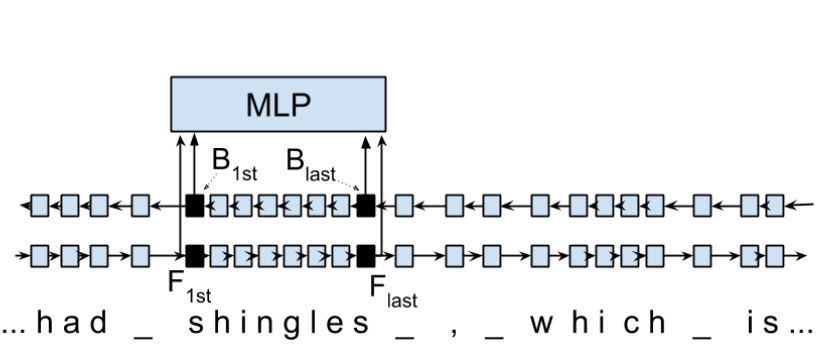
\includegraphics[width=.9\linewidth]{assets/nnfl1a.png}
\caption{Sentence-based Character Model: The representation for the token \emph{shingles} is the concatenation of the four shaded boxes.}
\end{figure}

For an \emph{n}-character sentence, for each character embedding \((e_{1}^{char},...,e_{n}^{char})\), a BiLSTM is applied:
\[
f_{c,i}^{0},b_{c,i}^{0} = BiLSTM(r_{0},(e_{1}^{char},...,e_{n}^{char}))_{i}
\]
For multiple layers(\emph{l}) that feed into each other through the concatenation of previous layer encodings, the last layer has both forward \((f_{c,l}^{l},...,f_{c,n}^{l})\) and backward \((b_{c,l}^{l},...,b_{c,n}^{l})\) output vectors for each character.

To create word encodings, relevant subsets of these context sensitive character encodings are combined which can then be used in a model that assigns morphosyntactic tags to each word directly or via subsequent layers. To accomplish this, the model concatenates upto four character output vectors: the \{\emph{forward, backward}\} output of the \{\emph{first, last}\} character in the token \emph{T} = \((F_{1st}(w), F_{last}(w), B_{1st}(w), B_{last}(w))\) which are represented by the four shaded box in \emph{Fig. 1}.

Thus, the proposed model concatenates all four of these and passes it as input to an multilayer perceptron (MLP):
\[
g_{i} = concat(T)
\]
\[
m_{i}^{chars} = MLP(g_{i})
\]
A tag can then be predicted with a \emph{linear classifier} that takes as input \(m_{i}^{chars}\), applies a \emph{softmax} function and chooses for each word the tag with highest probability.
\item Word-based Character Model
\label{sec:orgf269536}
To investigate whether a sentence sensitive character model (\emph{Fig.1}) is better than a model where the context is restricted to the characters of a word, (\emph{Fig.2}) which uses the final state of a unidirectional LSTM, combined with the attention mechanism of (ADD REF: cao rei) over all characters.

\begin{figure}[htbp]
\centering
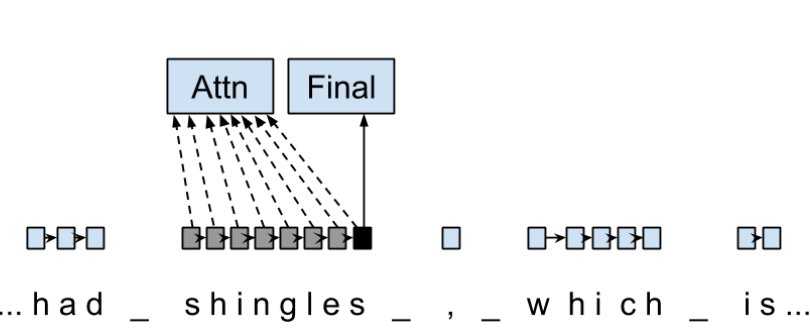
\includegraphics[width=.9\linewidth]{assets/nnfl1b.png}
\caption{Word-based Character Model: The token is represented by concatenation of attention over the lightly shaded boxes with the final cell (dark box).}
\end{figure}

\begin{figure}[htbp]
\centering
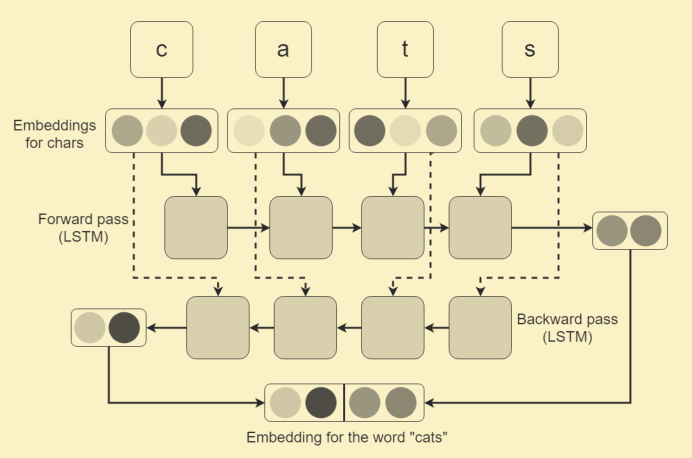
\includegraphics[width=.9\linewidth]{assets/nnfl1.png}
\caption{BiLSTM variant of Character-level word representation}
\end{figure}

\item Sentence-based Word Model
\label{sec:org6d063a4}
The inputs are the words of the sentence and for each of the words, we use pre-trained word embeddings \((p_{1}^{word},...,p_{n}^{word})\) summed with a dynamically learned word embedding for each word in the corpus \((e_{1}^{word},...,e_{n}^{word})\):
\[
in_{i}^{word} = e_{i}^{word}+p_{i}^{word}
\]
The summed embeddings \(in_{i}\) are passed as input to one or more BiLSTM layers whose output \(f_{w,i}^{l}, b_{w,i}^{l}\) is concatenated and used as the final encoding, which is then passed to an MLP:
\[
o_{i}^{word} = concat(f_{w,i}^{l}, b_{w,i}^{l})
\]
\[
m_{i}^{word} = MLP(o_{i}^{word})
\]
The output of this BiLSTM is essentially the Word-based Character Model before tag prediction, with the exception that the word-based character encodings are excluded.

\begin{figure}[htbp]
\centering
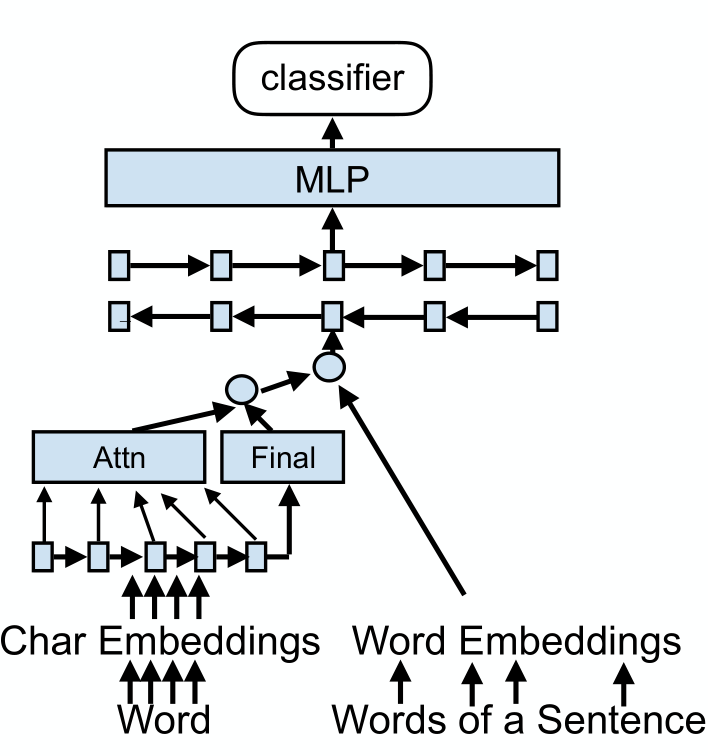
\includegraphics[width=.9\linewidth]{assets/nnfl2a.png}
\caption{Tagging Architecture of Word-based Character Model and Sentence-based Word Model}
\end{figure}

\item Meta-BiLSTM: Model Combination
\label{sec:orgabde472}
If each of the character or word-based encodings are trained with their own loss and are combined using an additional meta-BiLSTM model, optimal performance is obtained. The meta-biLSTM model concatenates the output of context sensitive character and word-based encoding for each word and puts this through another BiLSTM to create an \emph{additional} combined context sensitive encoding. This is followed by a final MLP whose output is passed to a linear layer for tag prediction.
\[
cw_{i} = concat(m_{i}^{char}, m_{i}^{word})
\]
\[
f_{m,i}^{l}, b_{m,i}^{l} = BiLSTM(r_{0},(cw_{0},...,cw_{n}))_{i}
\]
\[
m_{i}^{comb} = MLP(concat(f_{m,i}^{l}, b_{m,i}^{l}))
\]

\begin{figure}[htbp]
\centering
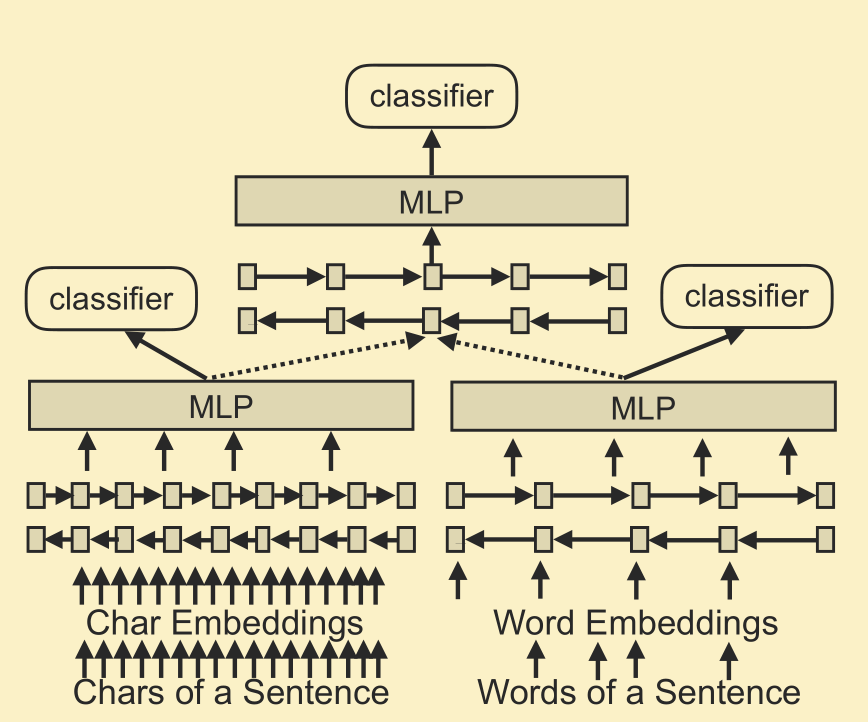
\includegraphics[width=.9\linewidth]{assets/nnfl2b.png}
\caption{Tagging Architecture of Meta-BiLSTM. Data flows along the arrows and the optimizers minimize the loss of the classifiers independently and backpropogate along the bold arrows.}
\end{figure}
\item Training Schema
\label{sec:org83e89f4}
Loss of each model is minimized independently by separate optimizers with their own hyperparameters which makes this a multi-task learning model and hence a schedule must be defined in which individual models are updated. In the proposed algorithm, during each epoch, each of the models are updated in sequence using the entire training data.

\begin{center}
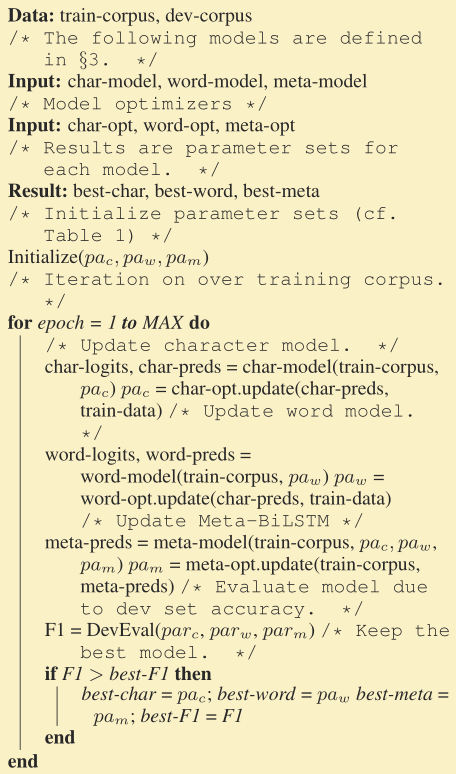
\includegraphics[width=.9\linewidth]{assets/nnflAlg.png}
\end{center}

In terms of model selection, after each epoch, the algorithm evaluates the tagging accuracy of the development set and keeps the parameters of the best model. Accuracy is measured using the meta-BiLSTM tagging layer, which requires a forward pass through all three models. Only the meta-BiLSTM layer is used for model selection and test-time prediction.

The training is synchronous as the meta-BiLSTM model is trained in tandem with the two encoding models, and not after they have converged. When the meta-BiLSTM was allowed to back-propagate through the whole network, performance degraded regardless of the number of loss functions used. Each language could in theory used separate hyperparameters but identical settings for each language works well for large corpora.
\end{enumerate}
\subsubsection{Experiments and Results}
\label{sec:orgf78b039}
\begin{enumerate}
\item Experimental Setup
\label{sec:orgfbe1c38}
The word embeddings are initialized with zero values and the pre-trained embeddings are not updated during training. The dropout\footnote{Dropping out units (hidden and visible) in a neural network, helps prevent the network from overfitting.} used on the embeddings is achieved by a single dropout mask and dropout is used on the input and the states of the LSTM.

\begin{table}[htbp]
\label{Architecture}
\centering
\begin{tabular}{llr}
Model & Parameter & Value\\
\hline
C,W & BiLSTM Layers & 3\\
M & BiLSTM Layers & 1\\
CWM & BiLSTM size & 400\\
CWM & Dropout LSTM & 0.33\\
CWM & Dropout MLP & 0.33\\
W & Dropout Embeddings & 0.33\\
C & Dropout Embedding & 0.5\\
CWM & Nonlinear Activation Fn (MLP) & ELU\\
\end{tabular}
\end{table}

TODO Add two remaining tables
\item Data Sets
\label{sec:org78e1783}
\item POS Tagging Results
\label{sec:org40f21d0}
\item POS Tagging on WSJ
\label{sec:org8018b89}
\item Morphological Tagging Results
\label{sec:orga971ce1}
\end{enumerate}
\subsubsection{Ablation Study (Takeaways)}
\label{sec:org16750c4}
\begin{itemize}
\item \textbf{Impact of the training schema}: Separate optimization better than Joint optimization
\item \textbf{Impact of the Sentence-based Character Model}: Higher accuracy than word-based character context
\item \textbf{Impact of the Meta-BiLSTM Model Combination}: Combined model has significantly higher accuracy than individual models
\item \textbf{Concatenation Strategies for the Context-Sensitive Character Encodings}: Model bases a token encoding on both forward and backward character representations of both first and last character in token. (\emph{Fig. 1}) \ldots{}.
\item \textbf{Sensitivity to Hyperparameter Search}: With larger network sizes, capacity of the network increases, but it becomes prone to overfitting. Future variants of this model might benefit from higer regularization.
\item \textbf{Discussion}: TODO Proposed modifications
\end{itemize}
\subsubsection{Conclusions}
\label{sec:orgc52981e}
\subsubsection{Readings and Resources}
\label{sec:org9e8719c}
\begin{enumerate}
\item Pytorch: \href{https://pytorch.org/tutorials/beginner/nn\_tutorial.html}{Beginner Guide}, \href{https://deeplizard.com/learn/playlist/PLZbbT5o\_s2xrfNyHZsM6ufI0iZENK9xgG}{Detailed Guides}, \href{https://www.cs.toronto.edu//\~lczhang/360/}{Notebook form}
\item Math: \href{https://explained.ai/matrix-calculus/index.html}{Matrix Calculus}, \href{https://mml-book.com/}{Book}
\item Basics:
\begin{itemize}
\item \href{https://www.kaggle.com/learn/python}{Python}
\item \href{https://realpython.com/jupyter-notebook-introduction/\#getting-up-and-running-with-jupyter-notebook}{Jupyter}
\item \href{http://cs231n.github.io/python-numpy-tutorial/\#numpy}{Numpy}, \href{https://nbviewer.jupyter.org/github/jrjohansson/scientific-python-lectures/blob/master/Lecture-2-Numpy.ipynb}{Numpy 2}
\item \href{https://mlcourse.ai/articles/topic1-exploratory-data-analysis-with-pandas/}{Pandas}, \href{https://www.kaggle.com/learn/pandas}{Pandas 2}
\item \href{https://mlcourse.ai/articles/topic2-visual-data-analysis-in-python/}{Matplotlib}, \href{https://matplotlib.org/matplotblog/posts/an-inquiry-into-matplotlib-figures/}{Matplotlib 2}
\item \href{https://mlcourse.ai/articles/topic2-part2-seaborn-plotly/}{Seaborn}
\item \href{http://scipy-lectures.org/}{Overview}
\end{itemize}
\item Interactive Tutorials on \href{https://www.deeplearning.ai/ai-notes/initialization/}{Weight Initialization}, \href{https://www.deeplearning.ai/ai-notes/optimization/}{Different Optimizers}
\item Rougier's Bits
\begin{itemize}
\item \href{https://github.com/rougier/matplotlib-tutorial}{Matplotlib Tutorial}, \href{https://github.com/matplotlib/cheatsheets}{Matplotlib Cheatsheets}
\item \href{https://github.com/rougier/numpy-tutorial}{Numpy Tutorial}, \href{https://www.labri.fr/perso/nrougier/from-python-to-numpy/}{From Python to Numpy}, \href{https://github.com/rougier/numpy-100}{100 Numpy Exercises}
\item \href{https://www.labri.fr/perso/nrougier/python-opengl/}{Python \& OpenGL for Scientific Visualization}, \href{https://github.com/rougier/scientific-visualization-book}{Scientific Visualization}
\end{itemize}
\item NLP: \href{https://github.com/microsoft/nlp-recipes}{Best Practices}, \href{https://nlpoverview.com/}{DL Techniques for NLP}
\item BiLSTM: \href{https://arxiv.org/pdf/1807.00818v1.pdf}{Improving POS tagging}
\item \href{https://github.com/google/meta\_tagger}{Implementation} of the paper
\end{enumerate}
\subsection{Creating a blog using ox-hugo, org mode and github pages}
\label{sec:org28d1a31}
I was going to make a post explaining how I made this blog but it was rendered pretty useless by \href{https://dev.to/usamasubhani/setup-a-blog-with-hugo-and-github-pages-562n}{this.} So yeah, I might archive this later.

\begin{enumerate}
\item Install hugo from your package manager.
\item Create a new site:
\begin{verbatim}
hugo new site blog
\end{verbatim}
\item Add a theme:
\begin{verbatim}
cd blog
git init
git submodule add <theme_url> themes/<name>
\end{verbatim}
\item Install ox-hugo in emacs
\begin{verbatim}
;; goes in packages.el
(package! ox-hugo)

;; goes in config.el
(use-package ox-hugo
  :after ox)
\end{verbatim}
\item TODO Explain the process of content and properties, tags etc.
\item Export
\item Config.toml (theme, title, url, publishdir, etc)
\item Run server, check localhost.
\item Push
\item Go to GitHub repository Settings > GitHub pages. Select /docs in Source.
\item Voila!
\end{enumerate}
\section{Readings}
\label{sec:org9638a9c}
\section{Resources}
\label{sec:orgb99acd8}
\section{Notes}
\label{sec:org35f98ca}
\subsection{Microprocessors and Interfacing}
\label{sec:org62bb8da}
\subsubsection{Programmer's Model 8086}
\label{sec:org1add51b}

\begin{center}
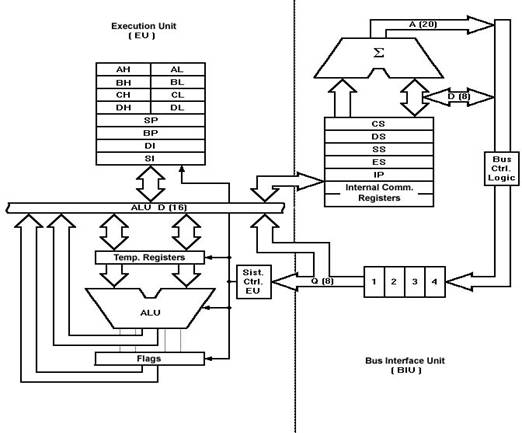
\includegraphics[width=.9\linewidth]{assets/8086model.png}
\end{center}
\subsection{Differential Geometry}
\label{sec:orgb0cc969}
\subsubsection{Theory of Space Curves}
\label{sec:orge27f023}
\begin{enumerate}
\item Representation of space curves
\label{sec:org62d7e26}
\begin{itemize}
\item Level Curve: f(x,y,z) = C
\item From level curves to parametrized curves:
\(y=x^{2} <-----> \gamma(t)=(\gamma_{1}(t),\gamma_{2}(t))\) Taking \(\gamma_{1}(t)=t\), we get \(\gamma_{2}(t)=t^{2}\) hence the parametrization is \(\gamma(t)=(t,t^{2})\)
\item \textbf{NOTE:} Check if domain of \emph{x} satisfies domain of \emph{t} or not. That is, the same parametrisation can be represented as \((t^{2}.t^{4})\) or \((t^{3},t^{6})\) but only the latter is a correct representation.
\item From parametrized curves to level curves:
\(\gamma(t)=(cos^{3}t,sin^{3}t)\) <------> F(x,y)=C; Using \(sin^{2}t+cos^{2}t=1\) we get, \(x^{2/3}+y^{2/3}=1\) as the level curve.
\end{itemize}
\item Unique Parametric representation
\label{sec:org9f4bb6f}
\begin{itemize}
\item Class 'm' \(\rightarrow\) \emph{f} is m-differentiable
\item A curve is \emph{smooth} if \(\frac{d^{n}f}{dt^{n}}\) exists for all n \(\ge\) 1 and t \(\in\) (\(\alpha\),\(\beta\))
\item A function \emph{f} is \emph{analytic} if it is single valued and of class \(\infty\)
\item A function is \emph{regular} if it is differentiable and derivative is non-zero (f dot \(\neq\) 0)
\item A \emph{regular f} of class \emph{m} can also be called a \emph{\textbf{path}} of class \emph{m}.
\item \textbf{NOTE:} A point of a parametrized curve can have multiple tangents.
\end{itemize}
\item Arc-length
\label{sec:org105fdef}
\begin{itemize}
\item Arc-length of a curve \(\gamma\) is given by the function \(s(t)=\int_{t_{0}}^{t}|| \dot{\gamma}(u)|| du\)
\item Speed: \(|| \dot{\gamma}(t) ||_{t}\) and a curve is unit-speed curve if its magnitude is 1 for all \emph{t}.
\item For \(\gamma\) being a unit speed curve, \(\ddot{\gamma}\) is zero or perpendicular to \(\dot{\gamma}\) i.e. \(\ddot{\gamma}.\dot{\gamma}=0\)
\item If \(\gamma\) is a regular curve, then its arclength S at any point of \(\gamma\) is a smooth function of t.
\item Reparametrization: \(\overline{\gamma}:(\overline{\alpha},\overline{\beta}) \rightarrow R^{n}\) <=> \(\gamma: (\alpha,\beta) \rightarrow R^{n}\)  exists iff \(\exists\) a smooth function \(\phi\): \((\overline{\alpha},\overline{\beta}) \rightarrow (\alpha,\beta)\) such that its inverse \(\phi\)\textsuperscript{-1} is also smooth.
\item A \emph{unit speed reparametrization} exists for a curve iff it is \emph{regular}.
\end{itemize}
\item Tangent and Osculating Plane
\label{sec:org6b529cd}
\begin{itemize}
\item Assuming \(\gamma\) is a class \(\ge\) 1 i.e. it has a power series expansion,
\end{itemize}
\[ \gamma(u)=\gamma(u_{0}+h)=\gamma(u_{0})+\frac{h}{1!}\dot{\gamma}(u_{0})+\frac{h^{2}}{2!}\ddot{\gamma}(u_{0})+ ... + \frac{h^{n}}{n!}\gamma^{n}(u_{0})+O(h^{n})
\]
  where \(h = u-u_0\)
\begin{itemize}
\item Let \(\gamma\) be class m \(\ge\) 2 and (P,Q) be points limiting position of a plane that contains tangential line at P and passes through Q as Q \(\rightarrow\) P is defined as the \emph{osculating plane}.
\item \textbf{Tangent line:} \(\vec{R}(t)=\vec{r}(u_{0})+t \vec{r'}(u_{0})\) at \(u_{0}\)
\item \textbf{Osculating Plane:} \([\vec{R}-\vec{r(0)}, \vec{r'(0)}, \vec{r''(0)}]=0\) where \(\vec{R}=(X,Y,Z)\) gives the equation of the OP (here \(\vec{r''}(0)\neq0\)). The product inside the box is \emph{scalar triple product}. Also, the OP passes through the unit vector of the curve and is perpendicular to the unit binormal vector.
\item Note that for smallest k \(\ge\) 2 such that \(\vec{r^{(k)}}=0\), the last term in the box is replaced by \(\vec{r'}^{(k)}(0)\)
\end{itemize}
\item Principal normal and binormal
\label{sec:org31d27a3}
\begin{itemize}
\item \textbf{Normal Plane:} \(\vec{t}(0).(\vec{R}-\vec{r}(0)) = 0\)
It is perpendicular to the tangent line and is spanned by \emph{n,b}
\item \textbf{Principal Normal Vector:} For m \(\ge\) 1, \(\vec{n}=\frac{\vec{r''}(0)}{||\vec{r''}(0)||}\)
\item \textbf{Unit Binormal Vector:} \(\vec{b}=\vec{t}\times\vec{n}\)
\item OP: b.(R-r)
\item NP: t.(R-r)
\item RP: n.(R-r)
\end{itemize}
\item Curvature and Torsion
\label{sec:org6bb063d}
\begin{itemize}
\item For a \emph{unit speed curve} or \emph{arc length parametrized} curve \(\gamma\)(t), the curvature \(\kappa\)(t) is defined as \(||\ddot{\gamma}(t)||\) (1)
\item For a \emph{regular} curve \(\gamma\)(t) \textbf{in} \(R^{3}\), \(\kappa = \frac{||\ddot{\gamma}\times\dot{\gamma}||}{||\dot{\gamma}^{3}||}\)
\item For a unit speed curve \(\gamma\), \emph{unit tangent vector} \(\hat{t}=\dot{\gamma}\) and for \(\kappa\) \(\neq\) 0, \emph{unit normal vector} is given by  \(\hat{n}(s)=\frac{\dot{\hat{\gamma}}(s)}{\kappa(s)}\) since (1). And \emph{unit binormal vector} can be given by \(\hat{b}=\hat{t}\times\hat{n}\)
\item \textbf{Orthonormal Basis} of a curve is given by \{\(\hat{t},\hat{n},\hat{b}\)\}
\item Now b is given by t \texttimes{} n , hence \(\dot{b}=\dot{t}\times n+t\times\dot{n}\) , since \(\dot{b}\) has to be perpendicular to t and b, \(\implies \ddot{b}||n\), therefore \(\boxed{\dot{b}=-\tau n}\) \textbf{iff} \(\kappa\) \(\neq\) 0.
\item Torsion measures the arc rate of turning of osculating plane.
\item For a regular curve \(\gamma\) in \(R^{3}\) with \(\kappa\) \(\neq\) 0, the \emph{torsion} is given by
\[
  \tau = \frac{(\dot{\gamma}\times\ddot{\gamma}).\dddot{\gamma}}{||\dot{\gamma}\times\ddot{\gamma}||^{2}}
  \]
\item Also, \emph{radius of curvature} \(\rho\) is inverse of curvature.
\item Finally, tying it all together is the \emph{Serret-Frenet formula} (arc length parameter):
\(\begin{bmatrix} \dot{t} \\
   \dot{n} \\
   \dot{b}  \end{bmatrix} = \begin{bmatrix} 0 & \kappa & 0 \\
    -\kappa & 0 & \tau \\
    0 & -\tau & 0 \end{bmatrix} \begin{bmatrix} t \\
    n \\
    b \end{bmatrix}\)
\end{itemize}
\item Behaviour of a curve near one of its points
\label{sec:org36547a3}
\begin{itemize}
\item For a regular curve of class m \(\ge\) 2 with nonvanishing curvature, the curve is \emph{planar} iff \(\tau\)=0 everywhere.
\item For an analytic curve with arc length parameter, as s \(\rightarrow\) 0, a new parametrization for small s can be defined as:
\[
    X = s - \frac{\kappa^{2}s^{3}}{6} - \frac{\kappa\kappa' s^{4}}{8} + o(s^{4})
  \]
\[
    Y = \frac{\kappa s^{2}}{2} + \frac{\kappa' s^{3}}{6} + \frac{\kappa''-\kappa\tau-\kappa^{3}}{24} s^{4} + o(s^{4})
  \]
\[
   Z = \frac{\kappa\tau}{6}s^{3} + \frac{2\kappa'\tau+\kappa\tau'}{24}s^{4} + o(s^{4})
  \]
\item Here the o notation represents that for f = o(g), as s \(\rightarrow\) 0, \(lim \frac{f(s)}{g(s)}=0\)
\item From previous theorem:
\begin{enumerate}
\item \(\kappa(0) = \lim_{s \to 0} \frac{2Y}{X^{2}}\)
\item \(\tau(0) = \lim_{s \to 0} \frac{3Z}{XY}\)
\item For \(P=\vec{r}(0), Q=\vec{r}(s)\), the length of chord
 \[
      PQ = s(1-\frac{\kappa^{2}s^{2}}{24}) + o(s^{3}) \~ s(1-\frac{\kappa^{2}s^{2}}{24})o(s^{3})
    \]
If f(t)=g(t)+o(t), then as t \(\rightarrow\) 0, it can be written as f(t)\textasciitilde{}g(t)o(t)
\end{enumerate}
\item The length of common perpendicular between tangents at two nearby points of \(\vec{r}(s)\) at arcual distance \emph{s} is approximately \(d=\frac{\kappa\tau s^{3}}{12}\). This is the shortest distance between tangents at nearby points of r(s).
\end{itemize}
\item Contact between curves and surface
\label{sec:org15fda41}
\begin{itemize}
\item For a surface S: F(x,y,z)=0 and a parametrized curve C: \(\vec{r}(u)\) = (f(u),g(u),h(u)), let P be a point on C. P lies on S iff F(f(P),g(P),h(P))=0.
\item Let \(\phi\)(u) = F(f(u),g(u),h(u)) for any parameter value u. Then P lies on S iff \(\phi\)(u\textsubscript{0})=0.
\item Assuming F and \(\vec{r}\) are of class m for sufficiently large m, then \(\phi\)(u) has a taylor expansion where \(\frac{O(h^{n+1})}{h^{n+1}}\) is bounded as h \(\rightarrow\) 0.
\item Definition: Surface S and a parametrized curve C has an \emph{n-point contact} (or contact of order n) at P if \(\phi(u_{0}) = \phi'(u_{0}) = ... = \phi^{(n-1)}(u_{0}) = 0\) and \(\phi^{(n)}(u_{0})\neq 0\)
\item If S and C have a contact of order 1 at P then it is called a \emph{simple intersection} of S and C.
\item If P is in n-point contact of S and C, then S and C intersect at P in \emph{n} coincidental points.
\item Condition for \emph{n-point contact} at P is invariant under a change of parameter.
\item Osculating Plane at P of \(\vec{r}\) has atleast a 3-point contact with \(\vec{r}\) at P.
\end{itemize}
\item Osculating circle (circle of curvature)
\label{sec:org29b498f}
\begin{itemize}
\item For a regular curve \(\vec{r}(s)\) of class m \(\ge\) 2, let \(P=\vec{r}(0)\) and \(P_{i}=\vec{r}(s_{i}), i=1,2,3\) be 3 non collinear points near P on the curve. Then there is a unique circle through all \(P_{i}\). The limiting circle, if existent, for all \(P_{i} \rightarrow P\) is called \emph{osculating circle} of r(s) at P.
\item Center of OC (c) is called \emph{centre of curvature} of r(s) at P while its radius \(\rho\)(0) is called radius of curvature. Also, the OC lies in the OP.
\item Theorem: \(\rho(0)=\frac{1}{\kappa(0)}\), \(\vec{c}(o)= \vec{r}(0)+\rho(0)\vec{n}(0)\)
\item OC does not exist at points where curvature vanishes and OC of a circle is the same circle itself.
\end{itemize}
\item Osculating Sphere
\label{sec:org7ad2fc0}
\begin{itemize}
\item Definition: For a regular path r(s) of class m \(\ge\) 2, assuming P = r(0) and \(\kappa\)(0)\(\tau\)(0) \(\neq\) 0, a sphere which has atleast a 4-point contact with r(s) at P is called \emph{osculating sphere} at P on r.
\item \(\rho\)(s)= \(\frac{1}{\kappa(s)}\) is called radius of curvature and \(\sigma\)(s)= \(\frac{1}{\tau(s)}\) is called radius of torsion of r(s)
\item Theorem: OS at P on r is given by \(|\vec{c}-\vec{R}|^{2} = R^{2}\) where \(R = \sqrt{\rho(0)^{2}+\sigma(0)^{2}\rho'(0)^{2}}\) and \(\vec{c}=\vec{r}(0)+\rho(0)\vec{n}(0)+\sigma(0)\rho'(0)\vec{b}(0)\) where c and R are COSC and ROSC to r(s) at r(0)
\item Centre of OS lies in the normal plane of r(s) as \(c-r(0)\) is a linear combination of n(0) and b(0)
\item If \(\kappa\) is constant then ROC=ROSC and COC=COSC. In particular, if r is a circle, then its its own OC and is a great circle of the OS.
\end{itemize}
\item Locus of centres of spherical curvature
\label{sec:org59b10d4}
\begin{itemize}
\item Since COSC at r(s) is \(c(s) =r(s)+\rho(s)n(s)+\sigma(s)\rho'(s)b(s)\), it moves along a path as \emph{s} varies. For this path, SFF, \(\kappa\), \(\tau\) can be calculated and will be denoted with subscript c.
\item Assuming \(\tau\)(s)>0,
\begin{enumerate}
\item \(c'(s) = (\frac{\rho(s)}{\sigma(s)}+ \frac{d (\sigma(s)\rho'(s))}{ds})b(s)\)
\item For a regular c(s), unit tangent vector is \(t_{c}(s) = eb(s)\)
\item \(\frac{ds_{c}}{ds}=|\frac{\rho(s)}{\sigma(s)}+\frac{d(\sigma(s)\rho'(s))}{ds}|\)
\end{enumerate}
Here e is 1 if ds\textsubscript{c}/ds > 0, -1 ow. Also \(e = t_{c}(s).b(s)\)
\item Also on differentiating,
\begin{enumerate}
\item \(\kappa_{c}(s) = \frac{\tau(s)}{\frac{ds_{c}}{ds}}\) or \(\kappa\)(s)= \(-\tau_{c}(s)e \frac{ds_{c}}{ds}\)
\item Which gives \(\tau(s)\tau_{c}(s)=\kappa(s)\kappa_{c}(s)\)
\end{enumerate}
\item Theorem: ROC of center of curvatures (i.e. center of OCs) is given by
\[
  \rho_{1} = [( \frac{\rho^{2}\sigma}{R^{3}}\frac{d}{ds}(\frac{\sigma\rho'}{\rho})-\frac{1}{R} )^{2} + \frac{\rho'^{2}\sigma^{4}}{\rho^{2}R^{4}}]^{-1/2}
  \]
\end{itemize}
\item Tangent surfaces, involutes and evolutes
\label{sec:org9374f1d}
\begin{itemize}
\item Definition: Tangent surface to a curve r is union of all tangent lines to r at all its points.
\item Tangent line to r at r(s) is R(u,s) = r(s)+ur'(s)
\item For both varying r and u, one gets the tangent surface.
\item Image of the curve u=u(s) in us-plane gives a curve \(r_{1}(s)=r(s)+u(s)r'(s)\)
\item Definition: Involute of r is a curve on the tangent surface of r which meets all generating lines orthogonally at corresponding points.
\item If \(r_{1}(s)\) denotes the pos vector on the involute C\textsubscript{1} of a curve C corresponding to its points r(s) then r\textsubscript{1}(s)=r(s)+(c-s)t(s) for a constant c.
\item For an involute c(s) of a regular path r(s) of class m \(\ge\) 2.
\[
    \kappa_{c}^2 = \frac{\tau^{2}+\kappa^{2}}{\kappa^{2}(c-s)^{2}}, \tau_c = \frac{\kappa\tau'-\kappa'\tau}{\kappa(c-s)(\tau^{2}+\kappa^{2})}
  \]

\item Definition: If \(\overline{C}\) is an involute of C then C is called an evolute of \(\overline{C}\).
\item For a regular curve r(s), evolute is given by \(r_{1}(s)=r(s)+\rho(s)n(s)+\rho(s)cot(\psi(s)+c)b(s)\) where c is a constant and \(\psi\)(s) = \(\int \tau(s)ds\)
\item r(s) has infinitely many evolutes, as c is random constant. For a plane curve, \(\tau\) = 0.
\item Tangents to two different evolutes corresponding to two constans A and B drawn from the same point of the given curve are inclined to each other at a constant angle A-B.
\[
    r_{1} = r+\rho\textbf{n}-\rho tan(\psi+a)\textbf{b}
  \]
Further \(\psi = \int \tau ds\) so that \(\psi\)'=\(\tau\)\ldots{}
\end{itemize}
\end{enumerate}
\subsubsection{First Fundamental Form and Local Intrinsic Properties of a Surface}
\label{sec:org85f63b3}
\begin{enumerate}
\item Introduction
\label{sec:org5146791}
\begin{itemize}
\item The surfaces are defined similar to curves by an equation of the type F(\emph{x,y,z}) = 0 or parametrically by expressing \emph{x,y,z} in terms of two parameters \emph{u,v} varying over a domain.
\item After defining the surface locally, its points are classified as ordinary or singular.
\item Then using tangent plane at a point and the surface normal at it, a coordinate system \textbf{\((r_1, r_2, N)\)} at every point of the surface is introduced.
\item After that, a certain quadratic differential form known as \emph{first fundamental form} on a surface and direction coefficients are introduced.
\end{itemize}
\item Definition of a Surface
\label{sec:orgacdc178}
\textbf{Definition 1:} Locus of a point P(\emph{x,y,z}) in \(E_{3}\) satisfying some restrictions on \emph{x,y,z} which is expressed by a relation of the type F(\emph{x,y,z}) = 0.

This equation is called the \emph{implicit} or the \emph{constraint} equation of the surface which allows for a global study of the surface.

\textbf{Definition 2:} For parameters \emph{u, v} taking real values and varying over a domain D, a surface is defined \emph{parametrically} as
  \[
      x = f(u,v), y = g(u,v), z = h(u,v)
  \]
  where \emph{f, g} and \emph{h} are single valued continuous functions possessing continuous derivatives of \emph{r}-th order. Such surfaces are called surfaces of class \emph{r}.

Parametric representation is useful for local study of surfaces i.e. in the neighbourhood of a point which is a small region \textbf{but} it is not unique for a surface. Also, the parameters \emph{u} and \emph{v} are called \emph{curvilinear coordinates}.

\textbf{Definition 3:} For two parametric representations \emph{u, v} and \emph{u', v'} of the same surface, any transformation of the form \(u'=\phi(u,v)\) and \(v'=\psi(u,v)\) relating the two representations is called a \emph{parametric transformation}.

\textbf{Definition 4:} A parametric transformation is \emph{proper} if:
\begin{enumerate}
\item \(\phi\) and \(\psi\) are single valued functions.
\item The Jacobian \(\frac{\delta (\phi,\psi)}{\delta (u,v)}\neq0\) in some domain D.
\end{enumerate}
These conditions are necessary and sufficient for existence of inverse in the neighbourhood of any point in D' which is the domain of \emph{u', v'} corresponding to the domain D of the \emph{u, v} plane.
\item Nature of Points on a Surface
\label{sec:org290f64c}
\textbf{Notation:} For \textbf{r} being the position vector of a point on the surface, \textbf{r} = (x,y,z), we can take r = r(u,v) as the parametric form of the surface and use \(r_1 = \frac{\delta r}{\delta u} = (x_{1},y_{1},z_{1})\) and \(r_2 = \frac{\delta r}{\delta v} = (x_{2},y_{2},z_{2})\), similarly we can denote second order derivatives using \(r_{11}, r_{21}\) etc.

\textbf{Definition 1:} If \(r_{1}\times r_{2}\neq0\) at a point on a surface, then the point is called an \emph{ordinary} point. A point which is not an ordinary point is called a \emph{singularity}.

Remarks:
\begin{itemize}
\item Considering M = \(\begin{bmatrix} x_{1} & y_{1} & z_{1}\\
  x_{2} & y_{2} & z_{2}\end{bmatrix}\)
For \(r_{1} \times r_{2} \neq 0\) at an ordinary point, i.e. rank of M is two at that point.
\item If the rank of M is either zero or one, the point on the surface is a singular point.
\item If \(r_{1} \times r_{2}\neq0\) or equivalently rank of M is two, then \emph{x,y,z} uniquely determine the parameters \emph{u,v} in the neighbourhood of an ordinary point.
\item When only one determinant minor of M is zero, one cannot conclude that the point is a singular point.
\item A \emph{proper} parametric transformation transforms an ordinary point into an ordinary point.
\item Due to geometrical nature of the surface, some singularities continue to be singularities, regardless of the parametric representations, these are called \emph{essential singularities}.
\item There are other singularities depending on the choice of parametric representation which are called \emph{artificial singularities}.
\end{itemize}
\textbf{Example:} Consider the circular cone represented by \emph{x = u sin\(\alpha\) cosv, y = u sin\(\alpha\) sinv, z = u cos\(\alpha\)} where \(\alpha\) is the semivertical angle of cone with O as origin and OP = \emph{u}, where P is any point on the cone.
Computing M, then at \emph{u} = 0, the determinant of every second order minor is zero, hence it is an essential singularity.

\textbf{Example:} Taking any point 0 as origin in the plane, \emph{x = u cosv, y = u sinv, z = 0}, we get \(r_{1} \times r_{2} = u\textbf{k}\). Hence it is zero only when \emph{u} = 0 i.e. it is an artificial singularity \emph{since} it arises due to the choice of the parametric coordinates and not due to the nature of the surface.
\item Representation of a Surface
\label{sec:orged47883}
For our study of surfaces, we consider only ordinary points. And we consider the entire surface as a collection of parts, each part being given a particular parametrisation and the adjacent parts being related by a \emph{proper} parametric transformation.

\textbf{Definition 1:} A representation R of a surface S of class \emph{r} in \(E_{3}\) is a collection of points in \(E_{3}\) covered by a system of overlapping parts \({S_{j}}\) where each part \{\{\(S_{j}\)\} is given by a parametric equation of class \emph{r}. Each point lying in the common portion of two parts \(S_{i}, S_{j}\) is such that the change of parameters from one part to is adjacent is given by a \emph{proper} parametric transformation of class \emph{r}.

\textbf{\emph{Note:}} Since one cannot parameterise the whole surface without introducing artificial singularities, one has to resort to a surface composed of many overlapping parts.

It is possible to have many representations of the same surface by considering different systems of overlapping parts (\(S_{j}\)), each part is given by a parametric equation of class \emph{r}.

\textbf{Definition 2:} For R and R' being two representations of class \emph{r} of the surface S, they are \emph{equivalent} if the composite family of parts \{\(S_{j},S'_{j}\)\} satisfies the condition that for each point P lying in the place of overlap, the change of parameter from \(S_{j}\)  to \(S'_{j}\) at P is given by a proper parametric transformation of class r.

\textbf{Theorem:} The notion of \emph{r}-equivalence of representations of a surface is an equivalence relation.

This equivalence relation introduces a partition into the family of surfaces of class \emph{r} splitting them into mutually disjoint equivalence classes, each class containing the surface equivalent to one another in the above equivalence relation.

\textbf{Definition 3:} A surface S of class \emph{r} in \(E_{3}\) is an \emph{r}-equivalence class of representations.

Thus a surface consists of different overlapping portions related to one another by proper parametric transformations and all other surfaces related to the given one by the equivalence relation of class \emph{r}.
\item Curves on Surfaces
\label{sec:orga8787e3}
For a surface \textbf{r} = r(\emph{u,v}), let \emph{u = u(t)} and \emph{v = v(t)} be a curve of class \emph{s} lying in the domain D of the \emph{uv}-plane. Considering \textbf{r} = r[u(t), v(t)] which gives the position vector of a point in terms of a single parameter \emph{t} such that it is a curve lying on a surface with class equal to the smaller of \emph{r} and \emph{s}. The equation \emph{u = u(t)} and \emph{v = v(t)} are called \emph{curvilinear equations} of the curve on the surface.

\textbf{Definition 1:} For \textbf{r}, a given surface of class \emph{r}, let \emph{v = c}, then position vector \textbf{r} = r(u,c) is a function of a single parameter \emph{t} and hence \textbf{r} = r(u,c) represents a curve lying on the surface \textbf{r} = r(u,v). This curve is called the \emph{parametric curve} v = constant.

By varying the values of \emph{c}, a system of parametric curves \emph{v} = constant is generated and similarly another system is generated by keeping \emph{u} constant and varying \emph{v}.

Properties that are a consequence of assuming only ordinary points on the surface:
\begin{enumerate}
\item Through every point of the surface, there passes one and only one parametric curve of each system.
\item No two curves of the same system intersect.
\item The curves of the system \(u=u_{o}\) and \(v=v_{o}\) intersect once but not more than once if \((u_{o},v_{o}) \in D\).
\item The parametric curves of the system u = \(c_{1}\) and v = \(c_{2}\) cannot touch each other.
\end{enumerate}

\textbf{Definition 2:} Let u = \(c_{1}\) and v = \(c_{2}\), when the constants vary, the whole surface is covered with a net of parametric curves, two of which pass through each point.

\textbf{Definition 3:} Two parametric curves through a point P are \emph{othogonal} if \(\textbf{r}_{1}.\textbf{r}_{2}= 0\) at P.
\item Tangent Plane and Surface Normal
\label{sec:orgc79e0b8}
Let \textbf{r} = r[u(t), v(t)] be a general curve lying on the surface passing through [u(t), v(t)], then the tangent to the curve at any point P on the surface is
\[
\frac{dr}{dt} = r_{1}\frac{du}{dt}+r_{2}\frac{dv}{dt}
\]
\textbf{Definition 1:} Tangent to any curve drawn on a surface is called a tangent line to the surface. The tangents to different curves through P on a surface lie in a plane containing two independent vectors \(r_{1}\) and \(r_{2}\) at P called the \emph{tangent plane} at P.

\textbf{Theorem 1:} The equation of a tangent plane at P on a surface with position vector \textbf{r} = r(u,v) is either \(R = r+ar_{1}+br_{2}\) or \((R-r).(r_{1}\times r_{2}) = 0\) where a and b are parameters.

\textbf{Definition 2:} The normal to the surface P is a line through P and perpendicular to the tangent plane at P.

\textbf{Theorem 2:} The equation of the normal \textbf{N} at a point P on the surface r = r(u,v) is \(R=r+a(r_{1}\times r_{2})\).

\textbf{Theorem 3:} A proper parametric transformation either leaves every normal unchanged or reverses the direction of the normal.
\item General Surface of Revolution
\label{sec:org6785d2f}
\textbf{Definiton 1:} A surface generated by the rotation of a plane curve about an axis in its plane is called a \emph{surface of revolution}.

\textbf{Theorem 1:} The position vector of any point on the surface of revolution generated by the curve [g(u),o,f(u)] in the XOZ plane is
\[
\textbf{r} = [g(u)cosv, g(u)sinv, f(u)]
\]
where \emph{v} is the angle of roatation about the \emph{z}-axis.
\end{enumerate}
Emacs 28.0.50 (Org mode 9.5)
\end{document}
